% Options for packages loaded elsewhere
\PassOptionsToPackage{unicode}{hyperref}
\PassOptionsToPackage{hyphens}{url}
\PassOptionsToPackage{dvipsnames,svgnames,x11names}{xcolor}
\documentclass[
  11pt,
]{article}
\usepackage{xcolor}
\usepackage[margin=1in]{geometry}
\usepackage{amsmath,amssymb}
\setcounter{secnumdepth}{-\maxdimen} % remove section numbering
\usepackage{iftex}
\ifPDFTeX
  \usepackage[T1]{fontenc}
  \usepackage[utf8]{inputenc}
  \usepackage{textcomp} % provide euro and other symbols
\else % if luatex or xetex
  \usepackage{unicode-math} % this also loads fontspec
  \defaultfontfeatures{Scale=MatchLowercase}
  \defaultfontfeatures[\rmfamily]{Ligatures=TeX,Scale=1}
\fi
\usepackage{lmodern}
\ifPDFTeX\else
  % xetex/luatex font selection
\fi
% Use upquote if available, for straight quotes in verbatim environments
\IfFileExists{upquote.sty}{\usepackage{upquote}}{}
\IfFileExists{microtype.sty}{% use microtype if available
  \usepackage[]{microtype}
  \UseMicrotypeSet[protrusion]{basicmath} % disable protrusion for tt fonts
}{}
\makeatletter
\@ifundefined{KOMAClassName}{% if non-KOMA class
  \IfFileExists{parskip.sty}{%
    \usepackage{parskip}
  }{% else
    \setlength{\parindent}{0pt}
    \setlength{\parskip}{6pt plus 2pt minus 1pt}}
}{% if KOMA class
  \KOMAoptions{parskip=half}}
\makeatother
\usepackage{longtable,booktabs,array}
\newcounter{none} % for unnumbered tables
\usepackage{calc} % for calculating minipage widths
% Correct order of tables after \paragraph or \subparagraph
\usepackage{etoolbox}
\makeatletter
\patchcmd\longtable{\par}{\if@noskipsec\mbox{}\fi\par}{}{}
\makeatother
% Allow footnotes in longtable head/foot
\IfFileExists{footnotehyper.sty}{\usepackage{footnotehyper}}{\usepackage{footnote}}
\makesavenoteenv{longtable}
\usepackage{graphicx}
\makeatletter
\newsavebox\pandoc@box
\newcommand*\pandocbounded[1]{% scales image to fit in text height/width
  \sbox\pandoc@box{#1}%
  \Gscale@div\@tempa{\textheight}{\dimexpr\ht\pandoc@box+\dp\pandoc@box\relax}%
  \Gscale@div\@tempb{\linewidth}{\wd\pandoc@box}%
  \ifdim\@tempb\p@<\@tempa\p@\let\@tempa\@tempb\fi% select the smaller of both
  \ifdim\@tempa\p@<\p@\scalebox{\@tempa}{\usebox\pandoc@box}%
  \else\usebox{\pandoc@box}%
  \fi%
}
% Set default figure placement to htbp
\def\fps@figure{htbp}
\makeatother
\setlength{\emergencystretch}{3em} % prevent overfull lines
\providecommand{\tightlist}{%
  \setlength{\itemsep}{0pt}\setlength{\parskip}{0pt}}
\usepackage{bookmark}
\IfFileExists{xurl.sty}{\usepackage{xurl}}{} % add URL line breaks if available
\urlstyle{same}
% fallback for those not using the hyperref driver hyperxmp:
\makeatletter
\@ifundefined{xmpquote}{\newcommand{\xmpquote}[1]{#1}}{}
\makeatother
\hypersetup{
  pdftitle={Who Gets Served When Capacity Is Scarce? Equity-Aware Optional-Service Routing for Food Redistribution in New York City},
  pdfauthor={Laidlaw Undergraduate Research Program},
  colorlinks=true,
  linkcolor={NavyBlue},
  filecolor={Maroon},
  citecolor={Blue},
  urlcolor={NavyBlue},
  pdfcreator={LaTeX via pandoc}}

\title{Who Gets Served When Capacity Is Scarce? Equity-Aware
Optional-Service Routing for Food Redistribution in New York City}
\author{Laidlaw Undergraduate Research Program}
\date{June 2026}

\begin{document}
\maketitle
\begin{abstract}
Food insecurity in New York City is spatially unequal, while the
transportation capacity, donated supply, and recipient opening windows
available to move rescued food are limited. When a fleet cannot serve
every recipient agency in a day, route planning becomes more than a
problem of minimizing distance. It also determines which neighborhoods
receive scarce food assistance, and the plan must adapt as donation
supply and recipient conditions are revealed during execution.

This paper frames urban food-rescue routing as an adaptive allocation
problem and formulates it as a three-layer model: a baseline
pickup-and-delivery vehicle-routing problem with time windows; a
food-rescue layer that adds cold-chain handling and an equity-weighted
value of serving each recipient; and a stochastic execution layer in
which donation supply is uncertain. The instance is a New York City
food-redistribution network built from public recipient-location data
and clearly labeled synthetic operating parameters. No individual
organization is named, evaluated, or used as the source of the
operational data. Recipient locations receive priority weights from two
distinct neighborhood conditions, estimated food need and spatial access
to existing assistance providers, and these weights enter the routing
objective as the modeled social value of serving each location. A
parameter controls the strength of equity prioritization, tracing the
tradeoff between the number of recipients served and service to
high-need, low-access communities.

We compare five strategies under identical vehicle, time, and supply
constraints: two benchmarks that carry no equity signal (an unweighted
benchmark and a random-preference benchmark), a need-only and an
access-only strategy, and the combined need-and-access strategy. Both
no-signal benchmarks leave the same neighborhoods underserved, reaching
about 31 percent of need-weighted demand, while the combined strategy
reaches about 45 percent under equal delivered volume by shifting
service toward high-need, low-access areas. An ablation shows that the
combined ratio outperforms either component alone on need-weighted
coverage, while a need-only objective best serves the single
highest-need tier. A parameter sweep exhibits diminishing marginal
equity gains beyond a moderate weighting level. The direction of these
effects is stable across perturbations to demand, travel times, opening
windows, and donation availability in the scenarios examined. The paper
demonstrates that routing objectives encode distributive choices and
provides a transparent framework for evaluating them. We frame recipient
receiving-capacity uncertainty and delivery recourse within the same
model and identify them as the principal direction for future work. The
model is intended as a strategic decision-support tool, not a substitute
for locally calibrated operational planning, and modeled service
coverage should not be read as a measurement of realized social impact.
\end{abstract}

\section{1. Introduction}\label{introduction}

\subsection{1.1 Scarcity makes routing an allocation
problem}\label{scarcity-makes-routing-an-allocation-problem}

Food insecurity persists in New York City even as large quantities of
edible food are discarded. Food-redistribution efforts recover surplus
food and deliver it to recipient agencies such as pantries, soup
kitchens, and meal programs. Across the five boroughs, on the order of a
million or more residents rely on this emergency food system, and need
is distributed unevenly: the neighborhoods with the highest
food-insecurity rates are frequently not the neighborhoods with the
densest networks of existing providers.

The fleet that moves rescued food is finite, and donated supply is
uncertain and often perishable. On any given day the fleet cannot reach
every recipient agency. This is the central observation of the paper:
when capacity is insufficient to serve all locations, routing is no
longer only a transportation problem. It is also an allocation problem,
because every feasible routing plan implicitly selects which communities
go unserved.

Common routing objectives are not neutral with respect to this
selection. Minimizing travel distance, maximizing pounds delivered, or
following an arbitrary or solver-determined visiting order each induces
a particular spatial distribution of service, usually without making
that distribution explicit. In the absence of an explicit distributive
objective, optional-service routing may prioritize locations according
to travel cost, demand size, or non-systematic operational habit rather
than community need.

\subsection{1.2 Execution-time uncertainty makes the allocation
adaptive}\label{execution-time-uncertainty-makes-the-allocation-adaptive}

The allocation a routing plan encodes is not fixed once the plan is
made. Food-rescue operations commit a plan before the day's conditions
are known and then adapt as those conditions are revealed. Two sources
of execution-time uncertainty are well documented in the literature
reviewed in Section 2. First, donated supply is uncertain: a donor
expected to contribute may bring less than planned or nothing at all, so
the food available to distribute is known only as the day unfolds.
Second, recipient organizations have limited and variable receiving
capacity: an agency may lack the storage, refrigeration, or staffing to
accept a full delivery on a given day, so food committed to a site may
not be placeable there. When either occurs, the plan must adapt, by
re-routing, partially delivering, or returning unplaced food to
warehouse cold storage for later redistribution. This adaptive response
is a form of recourse, and committing a route in advance and adapting it
under realized outcomes is the a-priori-routing-with-recourse paradigm
of stochastic vehicle routing.

The present paper develops the donation-supply form of this adaptation
directly: we commit each plan on expected supply and re-evaluate it
under sampled donation outcomes (Section 5.6). We formulate the
recipient-capacity and recourse forms within the same three-layer model
(Section 4.5) but leave their experimental evaluation to future work;
they are, in our view, the most promising next result the framework
points to.

\subsection{1.3 Thesis and research
question}\label{thesis-and-research-question}

These two observations combine into the thesis of the paper:

\begin{quote}
Under scarce capacity, urban food-rescue routing is an adaptive
allocation problem. The routing objective determines who is served,
which is a question of spatial equity, while uncertainty revealed during
execution, in donation supply and in recipient receiving-capacity,
forces the plan to adapt. A model that ignores either the distributive
choice or the execution-time adaptation misrepresents the system.
\end{quote}

The empirical core of the paper addresses the distributive half of this
thesis directly, through a question that is both operational and
normative:

\begin{quote}
When an urban food-redistribution network cannot serve all recipient
agencies, how does incorporating neighborhood need and spatial access
into an optional-service vehicle-routing model change the distribution
of service, and what efficiency cost does this impose?
\end{quote}

The phrase \emph{optional-service} is essential. Because supply and
fleet capacity are insufficient, recipient service is endogenous: the
model decides which locations to serve. The resulting problem is an
equity-weighted prize-collecting vehicle-routing problem with pickups,
deliveries, time windows, vehicle capacities, cold-chain compatibility,
and uncertain supply. The adaptive half of the thesis is developed
structurally: the three-layer model in Section 4 makes the adaptation
explicit, the donation-supply form is evaluated empirically, and
recipient-capacity recourse is set out as the principal extension
(Sections 4.5 and 7).

\subsection{1.4 Contributions}\label{contributions}

\begin{enumerate}
\def\labelenumi{\arabic{enumi}.}
\tightlist
\item
  \textbf{Framework.} We frame urban food-rescue routing as an adaptive
  allocation problem and organize it as a three-layer model, baseline
  routing, food-rescue structure with an explicit equity-weighted
  service value, and stochastic adaptive execution, and we position it
  against representative prior work in a feature-comparison table
  (Section 3).
\item
  \textbf{Modeling.} We formulate an equity-weighted optional-service
  pickup-and-delivery VRPTW in which recipient service is endogenous
  under scarce capacity, on a New York City network.
\item
  \textbf{Measurement.} We construct a transparent need-and-access
  priority measure that separates social need from existing provider
  availability, and we ablate its two components.
\item
  \textbf{Empirical.} We quantify the tradeoff between recipients
  served, travel cost, and distributional coverage on a reproducible NYC
  case network built from public and clearly labeled synthetic inputs.
\item
  \textbf{Robustness.} We test whether the direction of the equity
  effect persists under uncertainty in demand, travel time, service
  windows, and donation availability.
\end{enumerate}

\section{2. Operational motivation}\label{operational-motivation}

The modeling choices in this paper are motivated by features of
food-rescue logistics that are documented in the operations and
supply-chain literature. We summarize them here, drawn from published
accounts of the sector rather than from any single organization's
operational records.

\textbf{Routes combine many pickups with deliveries to heterogeneous
recipients.} Food rescue moves donated surplus from a changing set of
donors, such as supermarkets, wholesalers, and producers, to a mix of
recipient organizations including pantries, soup kitchens, shelters,
community sites, and mobile distributions. The resulting problem is a
pickup-and-delivery routing problem rather than a pure delivery problem,
and the recipient set is heterogeneous in size, schedule, and the
population it serves {[}4{]}, {[}2{]}.

\textbf{Donated supply is uncertain and perishable.} Donations are
committed informally and vary day to day; an expected donation may
shrink or fail to appear, and much rescued food is perishable and loses
value if it is delivered late or stored without refrigeration {[}2{]}.
Cold-chain handling and freshness are therefore first-order concerns,
not refinements.

\textbf{Recipient organizations have limited and variable receiving
capacity.} Recipient agencies differ in storage, refrigeration,
staffing, and opening hours, and these constraints bound how much food
an agency can accept on a given day. Models of equitable food
distribution and of food-bank supply chains treat recipient-side
capacity as a binding constraint {[}3{]}, {[}1{]}. Because that capacity
can be unknown until delivery is attempted, it is also a source of
execution-time uncertainty.

\textbf{Execution is adaptive, with recourse.} When supply or receiving
capacity differs from plan, the operation adapts: it re-routes, delivers
a partial quantity, moves food to another recipient, or returns unplaced
food to warehouse cold storage for later redistribution. Committing a
route in advance and adapting it as outcomes are realized is the
a-priori-routing-with-recourse design studied in stochastic vehicle
routing {[}7{]}.

Together these features motivate modeling food-rescue routing as a
stochastic, adaptive allocation problem with optional service,
cold-chain handling, uncertain donation supply, recipient
receiving-capacity, and recourse. The model in Section 4 incorporates
the first set of these features and donation-supply uncertainty
directly, and formulates recipient-capacity and recourse as the layer to
which the empirical study should extend next. We rely only on
documented, published features of the sector and on public
recipient-location data; no individual organization's private
operational information is used.

\section{3. Background and related
work}\label{background-and-related-work}

\textbf{Strategic food-supply-chain design.} A growing literature
optimizes food-redistribution systems at the strategic level, defining
social value in terms of beneficiaries served while confronting data
scarcity, heterogeneous capacities, and implementation constraints. That
work primarily concerns investment decisions. The present paper
addresses the corresponding operational allocation problem under fixed
resources.

\textbf{Operational food-rescue routing.} Models of donation pickup,
delivery, scheduling, and perishability show that nonprofit food
logistics cannot be treated as purely cost-driven, because donations are
uncertain, supply may fail to materialize, and much rescued food is
perishable. Our contribution is distinguished from this work as an
explicit treatment of spatial distributive equity when not every
recipient can be served.

\textbf{Equity and fairness in allocation.} Approaches to fairness in
distribution include proportional allocation, max-min fairness, and
need-weighted allocation, and a recurring theme is the tradeoff between
efficiency and equity. We encode equity as a need-weighted value of
service in the objective rather than as a hard constraint, which keeps
the formulation transparent and allows the strength of the equity
emphasis to be varied continuously.

\textbf{Spatial accessibility.} We measure access to existing providers
with the enhanced two-step floating catchment area (E2SFCA) method, a
standard accessibility approach that combines provider supply, local
demand, and distance decay. The method originated in healthcare access
analysis, so Section 4.4 states the adaptation explicitly.

\textbf{Positioning.} Table 1 positions the present paper against
representative prior work along the features identified in Section 2.
Two gaps stand out. First, no listed model combines an explicit
spatial-equity objective, built from neighborhood need and provider
access, with pickup-and-delivery routing under supply uncertainty; the
equity-aware allocation models do not route, and the routing models do
not encode spatial-access equity. Second, recipient-capacity uncertainty
together with recourse, the adaptive core of food-rescue execution, is
absent from all of them. The present paper closes the first gap and
formulates the second.

\textbf{Table 1. Feature comparison with representative prior work.}

{\def\LTcaptype{none} % do not increment counter
\begin{longtable}[]{@{}
  >{\raggedright\arraybackslash}p{(\linewidth - 12\tabcolsep) * \real{0.0909}}
  >{\centering\arraybackslash}p{(\linewidth - 12\tabcolsep) * \real{0.1515}}
  >{\centering\arraybackslash}p{(\linewidth - 12\tabcolsep) * \real{0.1515}}
  >{\centering\arraybackslash}p{(\linewidth - 12\tabcolsep) * \real{0.1515}}
  >{\centering\arraybackslash}p{(\linewidth - 12\tabcolsep) * \real{0.1515}}
  >{\centering\arraybackslash}p{(\linewidth - 12\tabcolsep) * \real{0.1515}}
  >{\centering\arraybackslash}p{(\linewidth - 12\tabcolsep) * \real{0.1515}}@{}}
\toprule\noalign{}
\begin{minipage}[b]{\linewidth}\raggedright
Feature
\end{minipage} & \begin{minipage}[b]{\linewidth}\centering
VRPTW {[}6{]}
\end{minipage} & \begin{minipage}[b]{\linewidth}\centering
HPDP {[}4{]}
\end{minipage} & \begin{minipage}[b]{\linewidth}\centering
Food rescue {[}2{]}
\end{minipage} & \begin{minipage}[b]{\linewidth}\centering
Equit. dist. {[}3{]}
\end{minipage} & \begin{minipage}[b]{\linewidth}\centering
Food-bank SC {[}1{]}
\end{minipage} & \begin{minipage}[b]{\linewidth}\centering
This paper
\end{minipage} \\
\midrule\noalign{}
\endhead
\bottomrule\noalign{}
\endlastfoot
Optional (prize-collecting) service & & $\checkmark$ & & $\checkmark$ & & $\checkmark$ \\
Pickup-and-delivery routing & & $\checkmark$ & $\checkmark$ & & & $\checkmark$ \\
Time windows & $\checkmark$ & & $\checkmark$ & & & $\checkmark$ \\
Cold-chain / perishability & & & $\checkmark$ & & & $\checkmark$ \\
Donation-supply uncertainty & & & $\checkmark$ & & & $\checkmark$ \\
Recipient receiving-capacity limits & & & & $\checkmark$ & $\checkmark$ & $\circ$ \\
Recipient-capacity uncertainty & & & & & & $\circ$ \\
Recourse / adaptive re-routing & & & & & & $\circ$ \\
Split / partial deliveries & & & & $\checkmark$ & & $\circ$ \\
Explicit equity objective & & $\checkmark$ & & $\checkmark$ & $\checkmark$ & $\checkmark$ \\
Spatial access measure & & & & & & $\checkmark$ \\
Real public-data instance & & & & $\checkmark$ & $\checkmark$ & $\checkmark$ \\
\end{longtable}
}

Key: VRPTW {[}6{]} is the time-window vehicle-routing benchmark; HPDP
{[}4{]} is the humanitarian pickup-and-distribution problem; Food rescue
{[}2{]} is donation pickup and delivery under uncertain, perishable
supply; Equit. dist. {[}3{]} is equitable distribution of donated food
under capacity constraints; Food-bank SC {[}1{]} is strategic food-bank
supply-chain design. A check mark ($\checkmark$) denotes a feature treated as a
modeled element of the cited work; a blank denotes a feature that is
absent or outside its scope; a circle ($\circ$) denotes a feature formulated
in the present model as an extension but not yet evaluated
experimentally (Sections 4.5 and 7). Entries reflect each work's primary
modeled scope and should be verified against the primary sources before
submission.

The gap we address empirically follows from the first column block.
Existing work shows that fairness can be incorporated into food
allocation and that pickup-and-delivery routing can reduce operating
costs. Less attention has been paid to the spatial question that arises
when service itself is optional: how should a routing model choose among
recipient locations when neighborhood need and provider access are
unequal? We address this question directly and treat the adaptive,
recipient-capacity-recourse extension as future work.

\section{4. The three-layer model}\label{the-three-layer-model}

\subsection{4.1 Case network and data
provenance}\label{case-network-and-data-provenance}

We study a New York City case network constructed from public
recipient-location data and practitioner-informed operating ranges. The
network has 528 recipient agencies with geographic coordinates and
opening hours across the five boroughs, a fleet of 25 heterogeneous
vehicles (about 70 percent refrigerated) operating from two depots, and
18 donor pickup locations, of which a subset are reliable and the
remainder are uncertain. Vehicles collect from donors and deliver to
recipients within a working day of about 14 hours, subject to time
windows, vehicle capacity, and cold-chain compatibility.

A core requirement for credibility is to distinguish what is observed
from what is assumed. Table 2 classifies every input. The recipient
locations and their opening hours are real NYC public data; the fleet,
depots, donors, and demand are synthetic scenario parameters chosen to
represent a plausible NYC operation. They are not drawn from, and should
not be read as, the operations of any specific organization.

\textbf{Table 2. Data provenance.}

{\def\LTcaptype{none} % do not increment counter
\begin{longtable}[]{@{}
  >{\raggedright\arraybackslash}p{(\linewidth - 4\tabcolsep) * \real{0.3333}}
  >{\raggedright\arraybackslash}p{(\linewidth - 4\tabcolsep) * \real{0.3333}}
  >{\raggedright\arraybackslash}p{(\linewidth - 4\tabcolsep) * \real{0.3333}}@{}}
\toprule\noalign{}
\begin{minipage}[b]{\linewidth}\raggedright
Input
\end{minipage} & \begin{minipage}[b]{\linewidth}\raggedright
Source type
\end{minipage} & \begin{minipage}[b]{\linewidth}\raggedright
Status
\end{minipage} \\
\midrule\noalign{}
\endhead
\bottomrule\noalign{}
\endlastfoot
Recipient locations (NYC) & Public & Observed \\
Opening schedules & Public & Observed, possibly outdated \\
Food-insecurity indicators & Public & Area-level estimate \\
Provider access score & Constructed & Model-derived (E2SFCA) \\
Recipient demand & Synthetic estimate & Assumed, calibrated to public
anchors \\
Vehicle fleet & Scenario parameter & Not an observed organizational
record \\
Donor supply and reliability & Synthetic, stochastic & Assumed \\
Depot locations & Scenario input & Representative, not an organizational
record \\
Travel times & Public road network plus calibration & Observed network,
calibrated congestion \\
\end{longtable}
}

\subsection{4.2 Overview of the three
layers}\label{overview-of-the-three-layers}

We build the model in three layers. Layer 1 is a baseline
pickup-and-delivery vehicle-routing problem with time windows and
capacities (Section 4.3). Layer 2 adds the structure specific to food
rescue: cold-chain handling and perishability, an explicit
equity-weighted value of serving each recipient built from neighborhood
need and access, and donor reliability (Section 4.4). Layer 3 adds
stochastic, adaptive execution: uncertain donation supply, and, as a
formulated extension, uncertain recipient receiving-capacity with
recourse (Section 4.5).

The layers differ in how far the present study takes them. Layers 1 and
2 are fully implemented and solved, except that recipient
receiving-capacity and split deliveries are formulated but not enforced
in the reported runs. In Layer 3 the donation-supply form of uncertainty
is implemented and evaluated (Section 5.6); recipient-capacity
uncertainty and recourse are formulated here but left to future work. We
flag this division explicitly so that the model's framing is not
mistaken for its evaluated scope.

\subsection{4.3 Layer 1: baseline pickup-and-delivery
VRPTW}\label{layer-1-baseline-pickup-and-delivery-vrptw}

Let \(O\) be depots, \(P\) donor pickup nodes, \(V\) recipient agencies,
and \(K\) vehicles, on a road network with arc travel times \(c_{ij}\).
Each recipient \(i\) has demand \(d_i\) and a time window
\([a_i, b_i]\); each donor \(p\) has an expected supply \(s_p\); each
vehicle \(k\) has total capacity \(Q_k\). Vehicles leave a depot, visit
a sequence of donor pickups and recipient deliveries within the working
day subject to capacity and time-window constraints, and return to the
depot. The baseline is thus a pickup-and-delivery vehicle-routing
problem with time windows.

Because total donated supply and fleet capacity are insufficient to
serve every recipient in a day, service is optional: a binary variable
\(y_i\) records whether recipient \(i\) is served, and the model selects
which recipients to visit. This optional, prize-collecting structure is
what turns routing into allocation, since every feasible plan leaves
some recipients unserved. The formal objective and constraints are
stated in Section 4.6.

\subsection{4.4 Layer 2: food-rescue structure and equity
prioritization}\label{layer-2-food-rescue-structure-and-equity-prioritization}

Layer 2 adds the structure that distinguishes food rescue from generic
routing.

\textbf{Cold-chain and perishability.} A share of each recipient's
demand is cold (refrigerated) demand. Vehicles carry a cold capacity
\(Q^{c}_k\) in addition to total capacity \(Q_k\), so refrigerated
demand can travel only on refrigerated vehicles, and a soft penalty
discourages late delivery of cold demand to capture freshness loss.
About 70 percent of the fleet is refrigerated and about 44 percent of
demand is cold in the case instance.

\textbf{Donor reliability.} Donors are heterogeneous in reliability: a
subset are reliable anchors, while the remainder are uncertain and may
supply less than expected or nothing at all. The expected supply \(s_p\)
is used at planning time; the realized supply is treated in Layer 3.

\textbf{Need and access measures.} For each NYC neighborhood we compute
two percentiles.

\emph{Need.} We use an area-level food-insecurity indicator as the need
percentile. This is a prevalence-based measure; it reflects the rate of
food insecurity in a neighborhood rather than the absolute count of
food-insecure residents. A population-weighted need measure would rank a
high-rate, low-population neighborhood differently from a lower-rate,
high-population one. Because population counts were not incorporated in
the present instance, we treat need as prevalence-based and note this as
a limitation.

\emph{Access.} We compute an access percentile using the E2SFCA method
over the recipient-provider set, weighting providers by their open
hours. Two adaptations of the original healthcare formulation should be
stated. First, provider capacity is approximated by opening hours rather
than measured throughput, so the result is an availability-based access
estimate rather than a complete measure of food access. Second, the
score is assigned to the neighborhood served by an agency, not to the
agency as an institution. There is a deliberate structural feature here:
provider locations both determine the access score and are the
destinations being routed to, so locations in provider-dense areas
receive lower priority. The model is therefore prioritizing
neighborhoods where the surrounding assistance infrastructure is sparse,
not judging the importance of any individual agency.

We refer to the resulting layer as a need-access priority surface. It is
a decision-support measure based on neighborhood averages. It is not an
individual-level assessment, not a complete measure of hunger, and
sensitive to data and parameter choices.

\textbf{Priority weight and the equity dial.} Each recipient i receives
a priority weight

\[ w_i \;=\; \operatorname{clip}\!\left(\left(\frac{N_i + \varepsilon}{A_i + \varepsilon}\right)^{\gamma},\; w_{\min},\; w_{\max}\right), \qquad \varepsilon = 0.15,\ \ [w_{\min}, w_{\max}] = [0.5, 4.0]. \]

Here \(N_i\) and \(A_i\) are the need and access percentiles. The ratio
encodes vertical equity: more value is placed on locations with greater
need and weaker existing access. The offset \(\varepsilon\) prevents the
ratio from diverging when access is near zero, and the clip bounds the
influence of any single location. Both are modeling choices rather than
neutral technical details; in our instance the weights take 128 distinct
values with median 0.96 and maximum 2.97, need and access percentiles
are only weakly correlated (\(r = 0.15\)), and a small share of
locations reach the clip bounds.

The exponent \(\gamma\) is the equity dial. It is a normative parameter
that expresses how strongly the system chooses to favor disadvantaged
neighborhoods, not a quantity to be estimated from data. At
\(\gamma = 0\) every weight equals one and the objective ignores equity.
At \(\gamma = 1\) the weight is the plain need-to-access ratio. As
\(\gamma\) increases the tilt sharpens. Section 5.5 traces the
consequences of each setting.

\textbf{Formulated extensions.} Two further food-rescue features are
formulated within this layer but not enforced in the reported runs.
First, recipient receiving-capacity: an agency can accept at most a
bounded quantity on a given day, which would cap delivered volume at a
site independently of vehicle capacity. Second, split or partial
deliveries: replacing the binary \(y_i\) with a delivered quantity
\(q_i \le d_i\) and a concave utility \(u(q_i / d_i)\), which would let
the model spread service across more sites. We return to both, and to
their stochastic counterparts, in Sections 4.5 and 7.

\subsection{4.5 Layer 3: stochastic and adaptive
execution}\label{layer-3-stochastic-and-adaptive-execution}

Layer 3 recognizes that a plan committed in the morning meets conditions
that are revealed only during execution.

\textbf{Uncertain donation supply (implemented).} We adopt an a-priori
design: each strategy commits its routes on expected donor supply, and
we then re-evaluate the committed plan under sampled donation outcomes
in which uncertain donors may deliver less than expected or nothing.
This yields a realized, as opposed to planned, coverage for each
strategy (Section 5.6). It is a commit-then-evaluate form of a-priori
routing: the plan is fixed and its performance is measured under
realized supply.

\textbf{Uncertain recipient capacity and recourse (formulated, future
work).} The same design extends naturally to the receiving side. If a
recipient's available capacity is uncertain and revealed only on
arrival, a committed plan may direct a vehicle to a site that cannot
accept its full delivery. A recourse rule would then adapt the plan:
deliver a partial quantity, carry the remainder to the next planned
site, or return unplaced food to warehouse cold storage for later
redistribution. Quantifying the cost of this recourse, namely the extra
travel incurred, the fraction of food returned to storage, and the
degradation in high-need coverage as the probability of a capacity
shortfall rises, is the most direct extension of the present results and
the principal item of future work. We note that this would simulate
recourse under an a-priori plan rather than solve the full two-stage
stochastic optimization, which is a recognized and tractable design
choice.

\subsection{4.6 The optional-service optimization
model}\label{the-optional-service-optimization-model}

Collecting the three layers, the decision variables are
\(x_{ijk} \in \{0,1\}\) for whether vehicle \(k\) traverses arc
\((i,j)\), \(y_i \in \{0,1\}\) for whether recipient \(i\) is served,
and cumulative load and time variables along each route. Because
capacity is insufficient to serve all recipients, \(y_i\) is endogenous.
We solve the prize-collecting form

\[ \max \;\; \sum_{i \in V} P\, w_i\, y_i \;-\; \lambda \sum_{k \in K} \sum_{(i,j)} c_{ij}\, x_{ijk} \;-\; \delta \sum_{i \in V} \text{cold}_i\, \tau_i, \]

where \(P\) is the base value of serving a location, \(w_i\) is the
Layer 2 priority weight, \(\lambda\) weights travel, \(\delta\)
penalizes late delivery of perishable (cold) demand to capture freshness
loss, and \(\tau_i\) is the arrival time at \(i\). This is equivalent to
minimizing travel plus a priority-weighted penalty for each unserved
location. The strategy is set entirely by the weights \(w_i\); all other
terms are held fixed across strategies.

The maximization is subject to standard constraints, stated in full in
Appendix A: degree and flow conservation linking \(x\) and \(y\) so that
a served recipient is visited exactly once; depot departure and return
for each vehicle; a load dimension in which donor visits add supply and
recipient visits subtract demand, bounded by \(Q_k\); a parallel
cold-load dimension bounded by \(Q^{c}_k\) so that refrigerated demand
travels only on refrigerated vehicles; time-window and route-duration
constraints; and optional, free visiting of donors, which are visited
only to enable deliveries.

The problem generalizes the prize-collecting vehicle-routing problem
with time windows, which is NP-hard, so we do not seek a provably
optimal solution. We solve with a constraint-programming routing solver
using guided local search under a fixed time budget. Two consequences
should be made explicit. First, when a recipient is served we deliver
its full estimated demand; the model selects locations rather than
partial quantities, the split-delivery relaxation noted in Section 4.4
being left to future work. Second, because the solver is heuristic,
reported values are bounded by a time budget rather than proven optimal,
so we emphasize relative comparisons across strategies solved under
identical conditions.

\subsection{4.7 Strategies compared}\label{strategies-compared}

All five strategies use the same network, fleet, and supply, and differ
only in the priority weight \(w_i\) that enters the objective. Holding
the rest of the model fixed isolates the effect of the objective. Two of
the strategies carry no equity signal and serve as benchmarks.

\textbf{Table 3. The five strategies.}

{\def\LTcaptype{none} % do not increment counter
\begin{longtable}[]{@{}
  >{\raggedright\arraybackslash}p{(\linewidth - 4\tabcolsep) * \real{0.3333}}
  >{\raggedright\arraybackslash}p{(\linewidth - 4\tabcolsep) * \real{0.3333}}
  >{\raggedright\arraybackslash}p{(\linewidth - 4\tabcolsep) * \real{0.3333}}@{}}
\toprule\noalign{}
\begin{minipage}[b]{\linewidth}\raggedright
Strategy
\end{minipage} & \begin{minipage}[b]{\linewidth}\raggedright
Weight \(w_i\)
\end{minipage} & \begin{minipage}[b]{\linewidth}\raggedright
Interpretation
\end{minipage} \\
\midrule\noalign{}
\endhead
\bottomrule\noalign{}
\endlastfoot
Unweighted & \(1\) & equal value to every recipient; selection driven by
routing cost and feasibility (a logistics-only benchmark) \\
Random-preference & \(\sim \operatorname{Uniform}(0.3, 1.7)\) &
arbitrary priorities with no equity signal; a stylized stand-in for
non-systematic operational choices such as visiting order or historical
habit \\
Need-only & need component, access held at its median & prioritizes
neighborhoods with greater estimated food need \\
Access-only & access component, need held at its median & prioritizes
neighborhoods with weaker access to existing assistance \\
Need-access & \(w_i\) from Section 4.4 & combines both dimensions (the
proposed weight) \\
\end{longtable}
}

The two benchmarks are mathematically distinct. The unweighted benchmark
values every recipient equally, so its selection is driven purely by
travel cost and feasibility. The random-preference benchmark assigns
each recipient an independent random value, so its selection follows an
arbitrary, non-systematic prioritization. We retain both because they
represent different ways a routing process can lack an equity signal,
and we do not claim that either exactly represents the practice of any
organization. The need-only and access-only strategies hold the other
component at its median value, so the three need-and-access strategies
share a common scale and form a clean ablation of the combined ratio.

\subsection{4.8 Evaluation}\label{evaluation}

We report five outcomes. Recipients served is the count of agencies
reached. Need-weighted coverage is the share of priority-weighted demand
that is met, using the combined weight as a fixed yardstick.
High-need-tier coverage is the share of demand met in the top tier of
the need percentile; unlike need-weighted coverage, this measure does
not use the access component, so it is a more neutral test of how a
strategy serves the neediest areas. Logistical cost is total vehicle
travel time. Finally, we re-evaluate each committed plan under sampled
donation outcomes to obtain a realized need-weighted coverage. We note
that need-weighted coverage is defined through the combined weight, so a
strategy optimizing that weight is expected to lead on it partly by
construction; the high-need-tier measure guards against reading too much
into that alignment.

\section{5. Results}\label{results}

\subsection{5.1 The priority surface}\label{the-priority-surface}

The need-access priority surface concentrates priority in NYC
neighborhoods that are high in need and low in access (Figure 1).
Because need and access are only weakly correlated, the ratio is not a
restatement of need alone, and the high-priority neighborhoods are
spatially clustered rather than uniformly distributed.

\begin{figure}
\centering
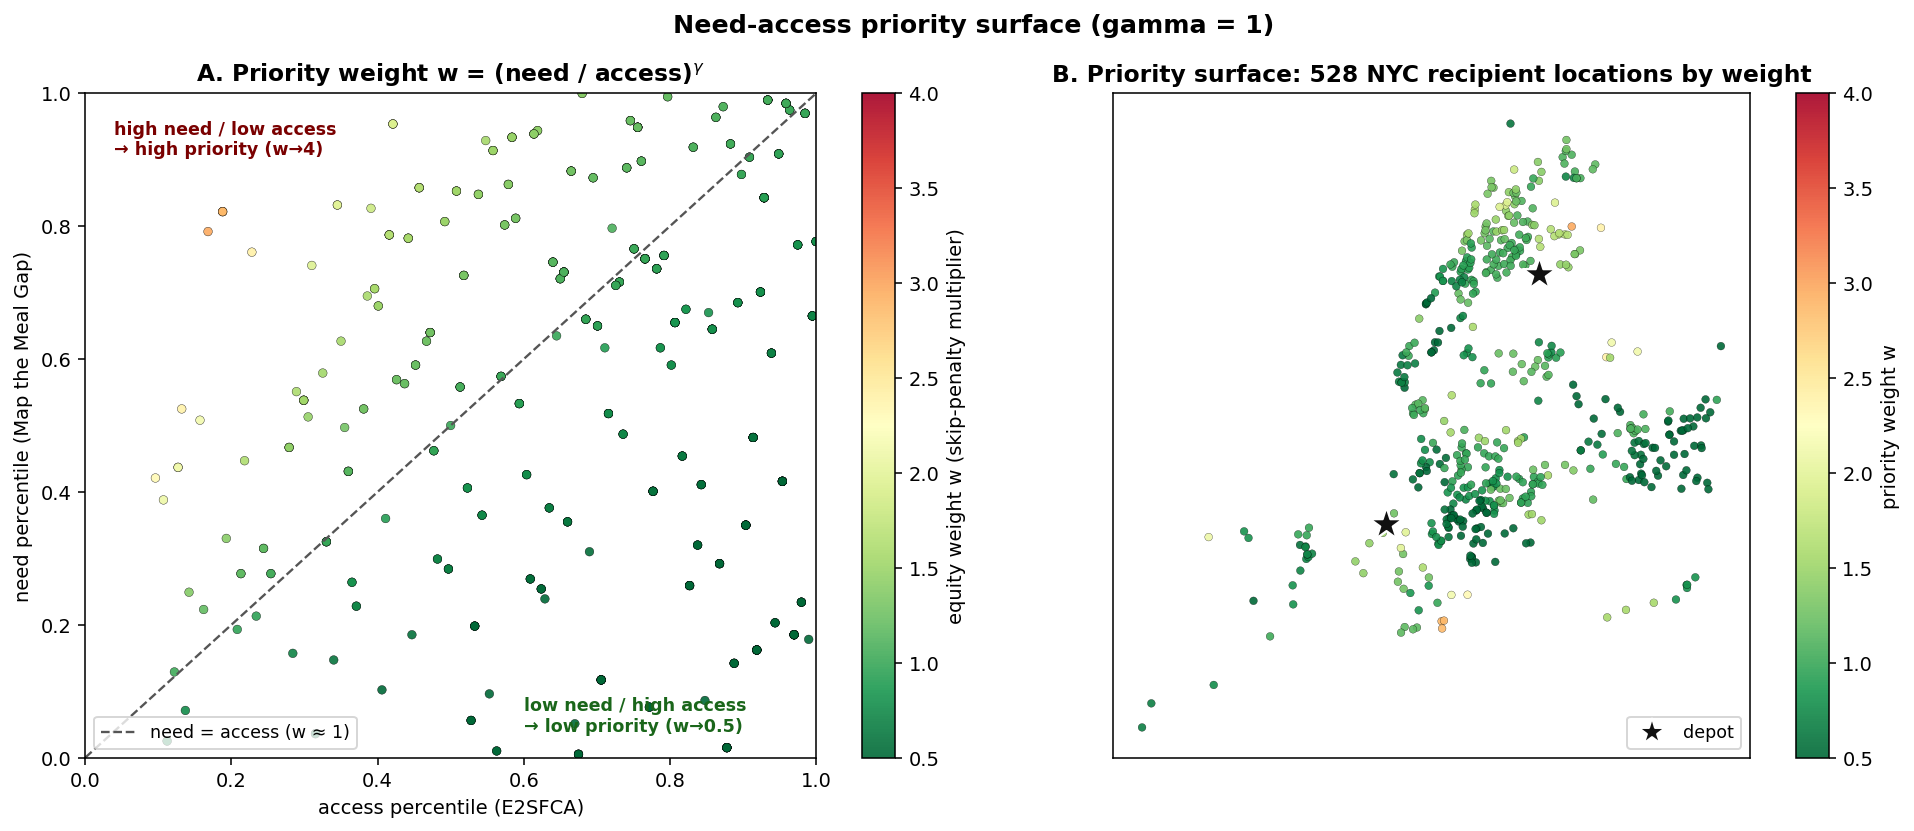
\includegraphics[width=0.92\linewidth,height=\textheight,keepaspectratio,alt={The need-access priority surface. Panel A places each recipient by access percentile (horizontal) and need percentile (vertical), colored by its priority weight; weights are largest in the high-need, low-access region. Panel B maps the same weights across the NYC recipient locations. High-priority locations cluster in particular neighborhoods.}]{fig_equity_layer.png}
\caption{The need-access priority surface. Panel A places each recipient
by access percentile (horizontal) and need percentile (vertical),
colored by its priority weight; weights are largest in the high-need,
low-access region. Panel B maps the same weights across the NYC
recipient locations. High-priority locations cluster in particular
neighborhoods.}
\end{figure}

\subsection{5.2 How the objective changes who is
served}\label{how-the-objective-changes-who-is-served}

The five strategies deliver nearly the same total food, because the
fleet is supply-limited, so the comparison is about where that food goes
rather than how much is moved. Table 4 reports the main outcomes, and
Figure 2 visualizes the tradeoff.

\textbf{Table 4. Strategy comparison on the NYC case network (fixed time
budget per solve).}

{\def\LTcaptype{none} % do not increment counter
\begin{longtable}[]{@{}
  >{\raggedright\arraybackslash}p{(\linewidth - 10\tabcolsep) * \real{0.1304}}
  >{\raggedleft\arraybackslash}p{(\linewidth - 10\tabcolsep) * \real{0.1739}}
  >{\raggedleft\arraybackslash}p{(\linewidth - 10\tabcolsep) * \real{0.1739}}
  >{\raggedleft\arraybackslash}p{(\linewidth - 10\tabcolsep) * \real{0.1739}}
  >{\raggedleft\arraybackslash}p{(\linewidth - 10\tabcolsep) * \real{0.1739}}
  >{\raggedleft\arraybackslash}p{(\linewidth - 10\tabcolsep) * \real{0.1739}}@{}}
\toprule\noalign{}
\begin{minipage}[b]{\linewidth}\raggedright
Metric
\end{minipage} & \begin{minipage}[b]{\linewidth}\raggedleft
Unweighted
\end{minipage} & \begin{minipage}[b]{\linewidth}\raggedleft
Random-pref.
\end{minipage} & \begin{minipage}[b]{\linewidth}\raggedleft
Need-only
\end{minipage} & \begin{minipage}[b]{\linewidth}\raggedleft
Access-only
\end{minipage} & \begin{minipage}[b]{\linewidth}\raggedleft
Need-access
\end{minipage} \\
\midrule\noalign{}
\endhead
\bottomrule\noalign{}
\endlastfoot
Recipients served & 237 & 229 & 209 & 200 & 184 \\
Need-weighted coverage \% & 31.1 & 30.8 & 36.9 & 41.0 & \textbf{44.8} \\
High-need-tier coverage \% & 29 & 24 & \textbf{60} & 24 & 44 \\
Tier coverage, low / mid / high \% & 22 / 45 / 29 & 49 / 37 / 24 & 1 / 8
/ 60 & 38 / 47 / 24 & 7 / 30 / 44 \\
Total delivered (lb) & 33,734 & 34,249 & 34,379 & 34,620 & 33,854 \\
Travel (vehicle-minutes) & 11,743 & 13,825 & 12,626 & 13,673 & 12,951 \\
\end{longtable}
}

Three findings stand out. First, the two benchmarks without an equity
signal land in nearly the same place on equity: the unweighted benchmark
reaches 31.1 percent of need-weighted demand and the random-preference
benchmark 30.8 percent, despite being built on entirely different
selection mechanisms. Whether recipients are chosen to minimize travel
or chosen arbitrarily, the result for high-need neighborhoods is
essentially the same. This convergence is the core point: without an
explicit equity signal, the routing objective does not serve high-need
areas, regardless of how the unserved are chosen.

Second, the random-preference benchmark is also the least
travel-efficient strategy (13,825 vehicle-minutes against 11,743 for the
unweighted benchmark), because arbitrary priorities pull vehicles toward
scattered locations. Lacking an equity signal does not buy logistical
efficiency in return.

Third, the combined need-access strategy produces the highest
need-weighted coverage (44.8 percent), well above either benchmark, by
reallocating service out of low-need areas and into high-need ones, as
Panel A of Figure 2 shows. It serves fewer recipients (184) to do so;
the benchmarks and the access-only strategy lie at the high-reach,
low-equity end of the frontier in Panel B.

\begin{figure}
\centering
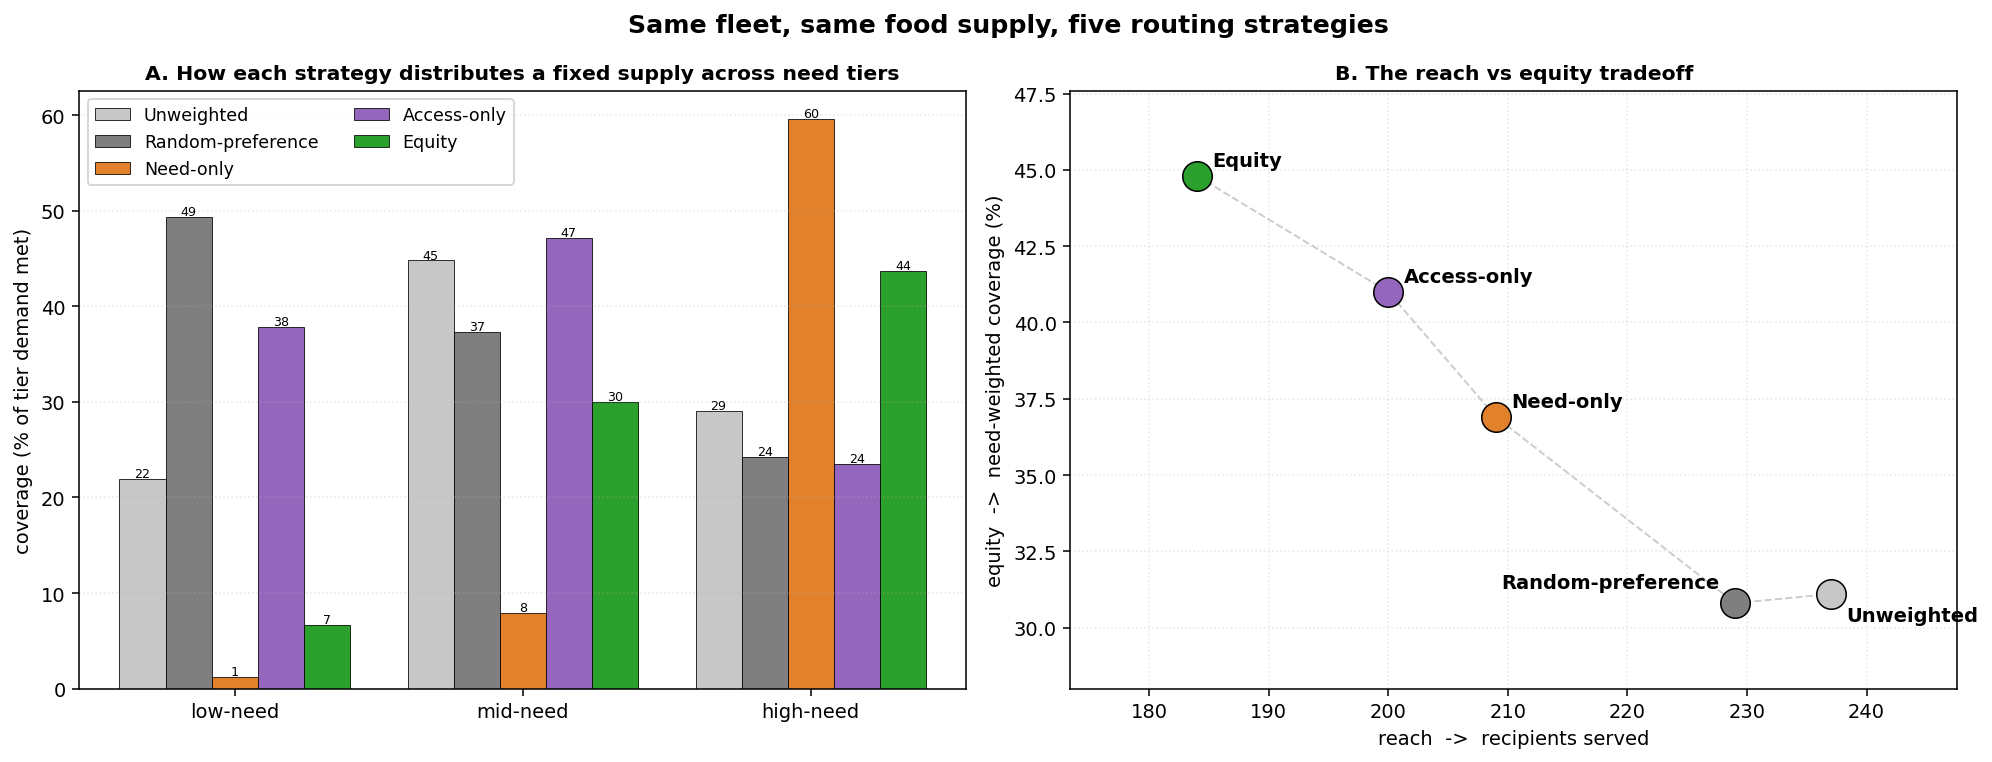
\includegraphics[width=0.92\linewidth,height=\textheight,keepaspectratio,alt={Same fleet and supply, five strategies. Panel A: coverage by need tier, showing how each objective distributes a fixed supply. Panel B: the reach-versus-equity tradeoff, with each strategy as a point. Higher need-weighted coverage comes at the cost of serving fewer recipients; the two no-signal benchmarks sit together at the low-equity end.}]{fig_tradeoff.png}
\caption{Same fleet and supply, five strategies. Panel A: coverage by
need tier, showing how each objective distributes a fixed supply. Panel
B: the reach-versus-equity tradeoff, with each strategy as a point.
Higher need-weighted coverage comes at the cost of serving fewer
recipients; the two no-signal benchmarks sit together at the low-equity
end.}
\end{figure}

To confirm that this is reallocation rather than an artifact of one
strategy moving more food, we re-solved with every strategy constrained
to deliver the same total volume. The gaps persist: under equal
delivered volume the need-access strategy meets about 44 percent of
need-weighted demand against about 31 percent for each benchmark, and
about 43 percent of the highest-need tier against about 25 to 28
percent.

\subsection{5.3 The model operationally: an illustrative route
map}\label{the-model-operationally-an-illustrative-route-map}

Aggregate coverage statistics can obscure what the model actually does
on the ground. Figure 3 shows a single illustrative solution for the NYC
network under the need-access strategy: vehicles leave the depots,
collect at donor pickup points, and deliver to the recipients selected
for service, following real road paths. The served recipients are the
green points; every grey point is a recipient the fleet did not reach
that day. That set of unserved points is precisely the distributive
consequence of the objective, made visible.

\begin{figure}
\centering
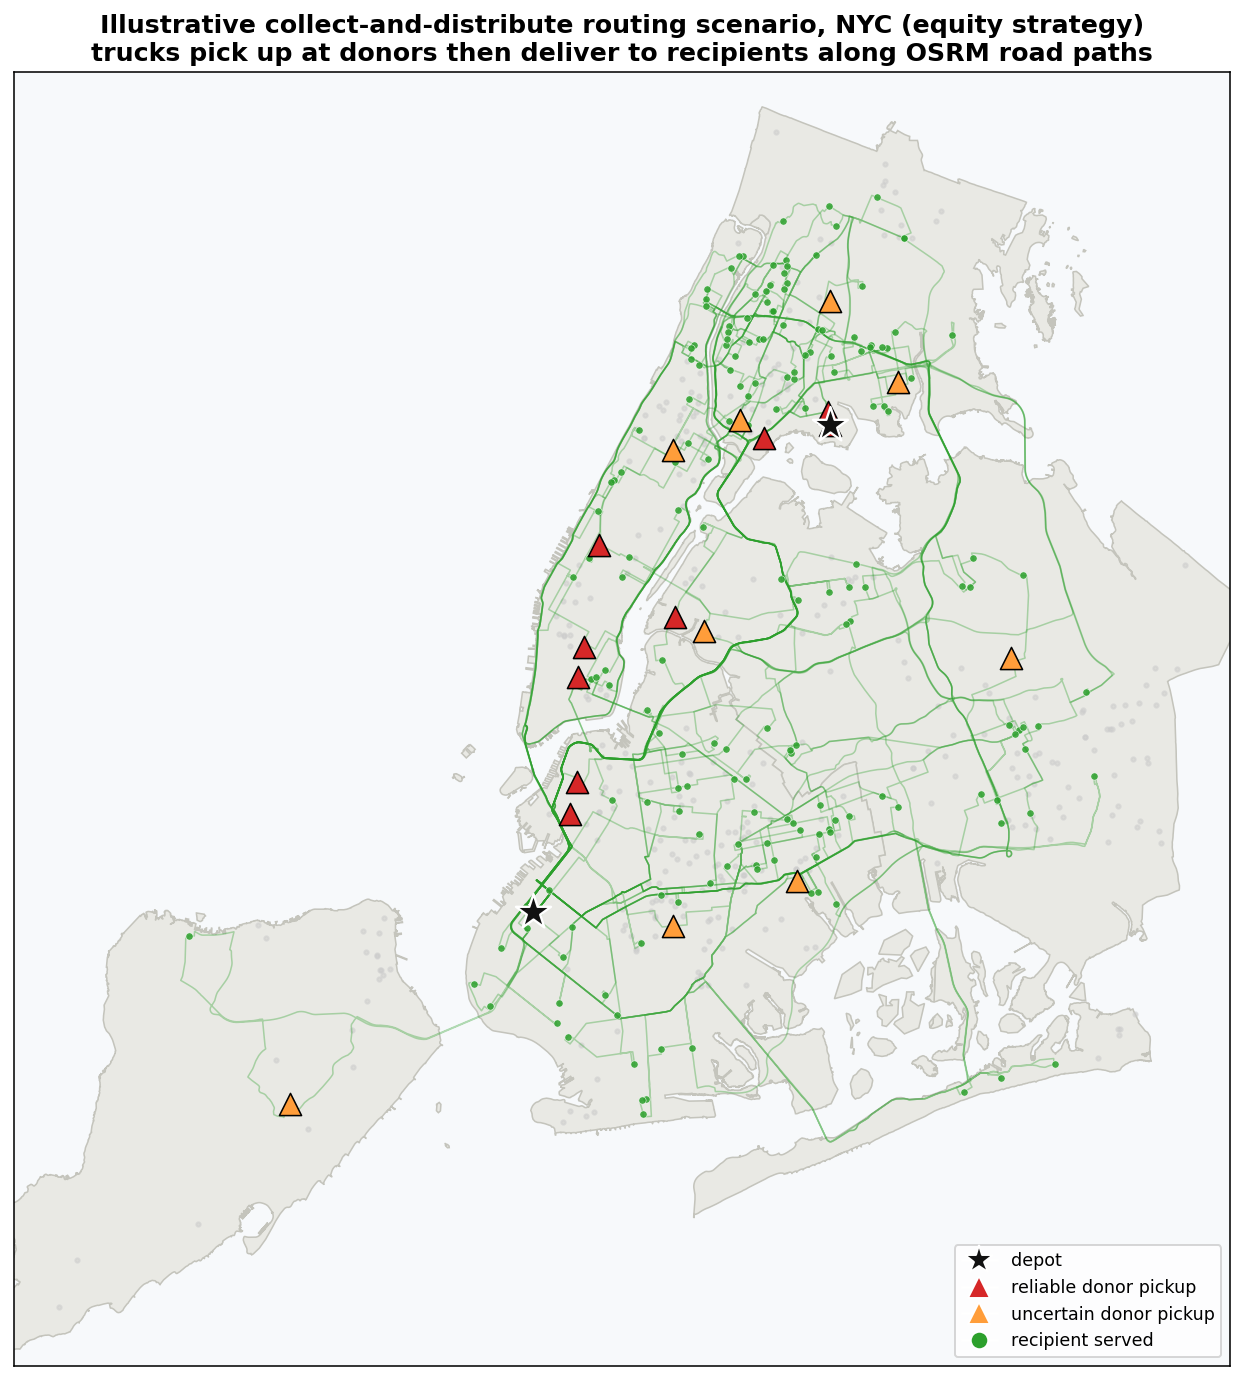
\includegraphics[width=0.92\linewidth,height=\textheight,keepaspectratio,alt={An illustrative collect-and-distribute routing solution for the NYC network under the need-access strategy. Stars are depots; triangles are donor pickup locations (reliable and uncertain, shown without identifying any specific donor); green points are recipients served; routes follow OSRM road paths. The figure is a modeled, illustrative scenario produced by the optimization model, not an observed route of any organization.}]{route_map_pickup.png}
\caption{An illustrative collect-and-distribute routing solution for the
NYC network under the need-access strategy. Stars are depots; triangles
are donor pickup locations (reliable and uncertain, shown without
identifying any specific donor); green points are recipients served;
routes follow OSRM road paths. The figure is a modeled, illustrative
scenario produced by the optimization model, not an observed route of
any organization.}
\end{figure}

\subsection{5.4 Ablation: does combining need and access add
information?}\label{ablation-does-combining-need-and-access-add-information}

The need-only and access-only strategies separate the two components of
the priority weight. The combined ratio gives higher need-weighted
coverage (44.8 percent) than either need alone (36.9 percent) or access
alone (41.0 percent), which indicates that the two components carry
partly independent information and that combining them is not redundant.

The picture differs for the single highest-need tier. There, the
need-only objective is strongest (60 percent coverage in Table 4, and
about 60 percent under equal volume), because it targets need directly,
while the combined ratio dilutes need-targeting with the access term and
reaches about 44 percent. Access alone is weakest on the high-need tier
(24 percent), since low access does not coincide with high need. In
short, the combined ratio is the best objective for need-weighted
coverage, whereas a need-only objective is preferable if the explicit
goal is to maximize service to the single neediest tier. This
distinction is a normative choice about what equity should mean, and the
framework makes it visible rather than resolving it by default.

\subsection{5.5 The equity dial}\label{the-equity-dial}

Sweeping \(\gamma\) from zero upward traces how prioritization
strengthens with the equity weight (Table 5, Figure 4). Moving from
\(\gamma = 0\) to \(\gamma = 0.25\) captures most of the available gain
at once, raising high-need-tier coverage from about 27 to 40 percent and
need-weighted coverage from about 31 to 41 percent, while recipients
served fall only modestly. Beyond \(\gamma \approx 1\) the equity
measures change little while reach continues to erode. The tested
instance therefore exhibits diminishing marginal gains between
\(\gamma = 0.5\) and \(\gamma = 1\). The preferred setting remains a
normative decision and may vary across networks.

\textbf{Table 5. Sweeping the equity dial.}

{\def\LTcaptype{none} % do not increment counter
\begin{longtable}[]{@{}
  >{\raggedleft\arraybackslash}p{(\linewidth - 6\tabcolsep) * \real{0.2500}}
  >{\raggedleft\arraybackslash}p{(\linewidth - 6\tabcolsep) * \real{0.2500}}
  >{\raggedleft\arraybackslash}p{(\linewidth - 6\tabcolsep) * \real{0.2500}}
  >{\raggedleft\arraybackslash}p{(\linewidth - 6\tabcolsep) * \real{0.2500}}@{}}
\toprule\noalign{}
\begin{minipage}[b]{\linewidth}\raggedleft
gamma
\end{minipage} & \begin{minipage}[b]{\linewidth}\raggedleft
Recipients served
\end{minipage} & \begin{minipage}[b]{\linewidth}\raggedleft
High-need-tier coverage \%
\end{minipage} & \begin{minipage}[b]{\linewidth}\raggedleft
Need-weighted coverage \%
\end{minipage} \\
\midrule\noalign{}
\endhead
\bottomrule\noalign{}
\endlastfoot
0.0 & 237 & 26.7 & 30.9 \\
0.25 & 196 & 39.8 & 40.6 \\
0.5 & 187 & 42.1 & 42.7 \\
1.0 & 183 & 47.3 & 46.5 \\
2.0 & 175 & 46.7 & 47.9 \\
3.0 & 178 & 45.8 & 47.7 \\
\end{longtable}
}

\begin{figure}
\centering
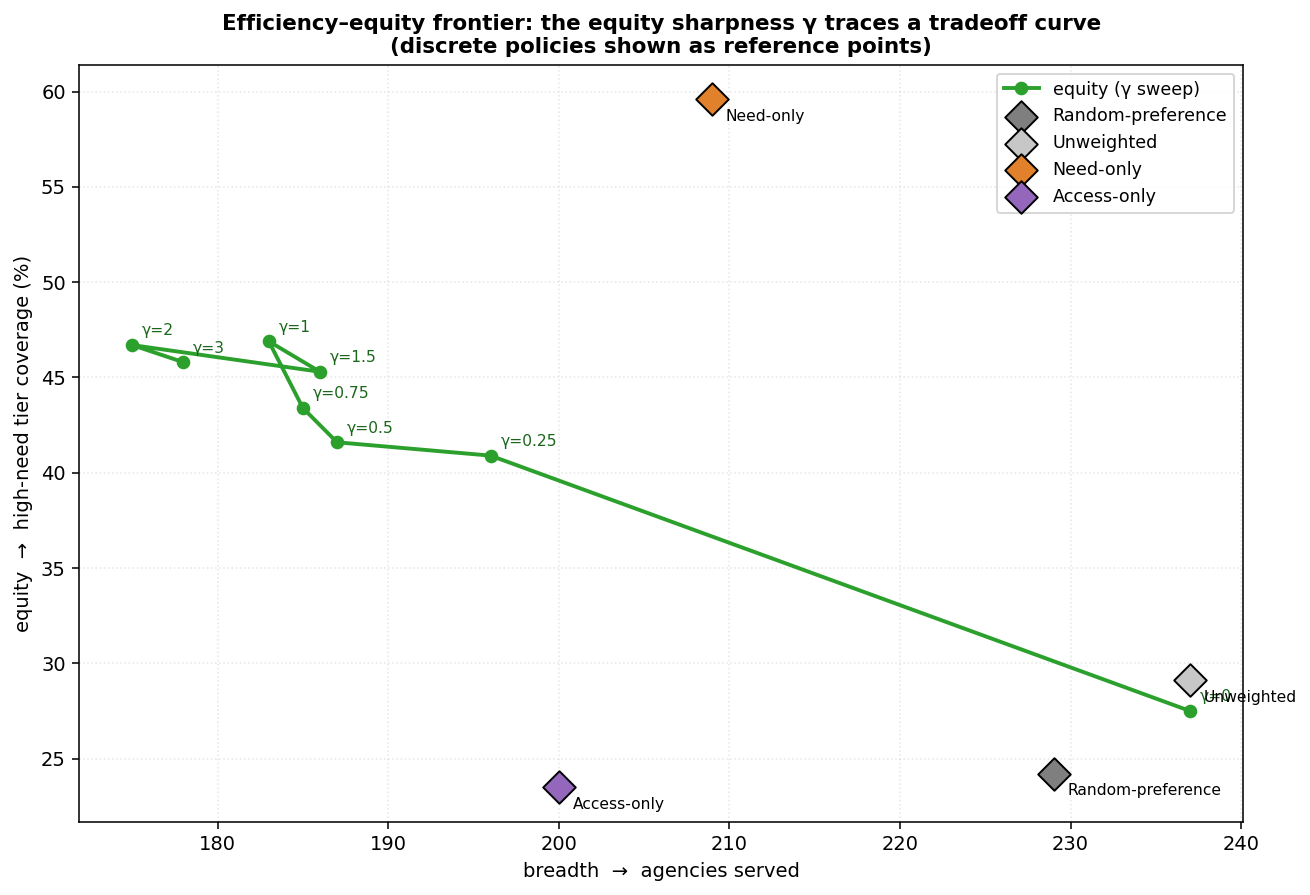
\includegraphics[width=0.92\linewidth,height=\textheight,keepaspectratio,alt={The equity dial as a frontier. The curve traces the need-access strategy as gamma varies from 0 to 3, with recipients served on the horizontal axis and high-need-tier coverage on the vertical axis. The other four strategies appear as reference points. Most of the equity gain is captured by a moderate gamma, after which the curve flattens.}]{pareto_frontier.png}
\caption{The equity dial as a frontier. The curve traces the need-access
strategy as gamma varies from 0 to 3, with recipients served on the
horizontal axis and high-need-tier coverage on the vertical axis. The
other four strategies appear as reference points. Most of the equity
gain is captured by a moderate gamma, after which the curve flattens.}
\end{figure}

\subsection{5.6 Robustness to
uncertainty}\label{robustness-to-uncertainty}

Two forms of uncertainty matter for a real system: donations may fail to
arrive, and the input data is imperfect.

\textbf{Donation uncertainty.} We committed each strategy's routes on
expected supply and then evaluated them over 120 sampled outcomes in
which unreliable donors may bring nothing. This lowered need-weighted
coverage by roughly 2 to 3 points for every strategy, by a similar
amount across strategies, so the relative ordering was preserved (Figure
5).

\begin{figure}
\centering
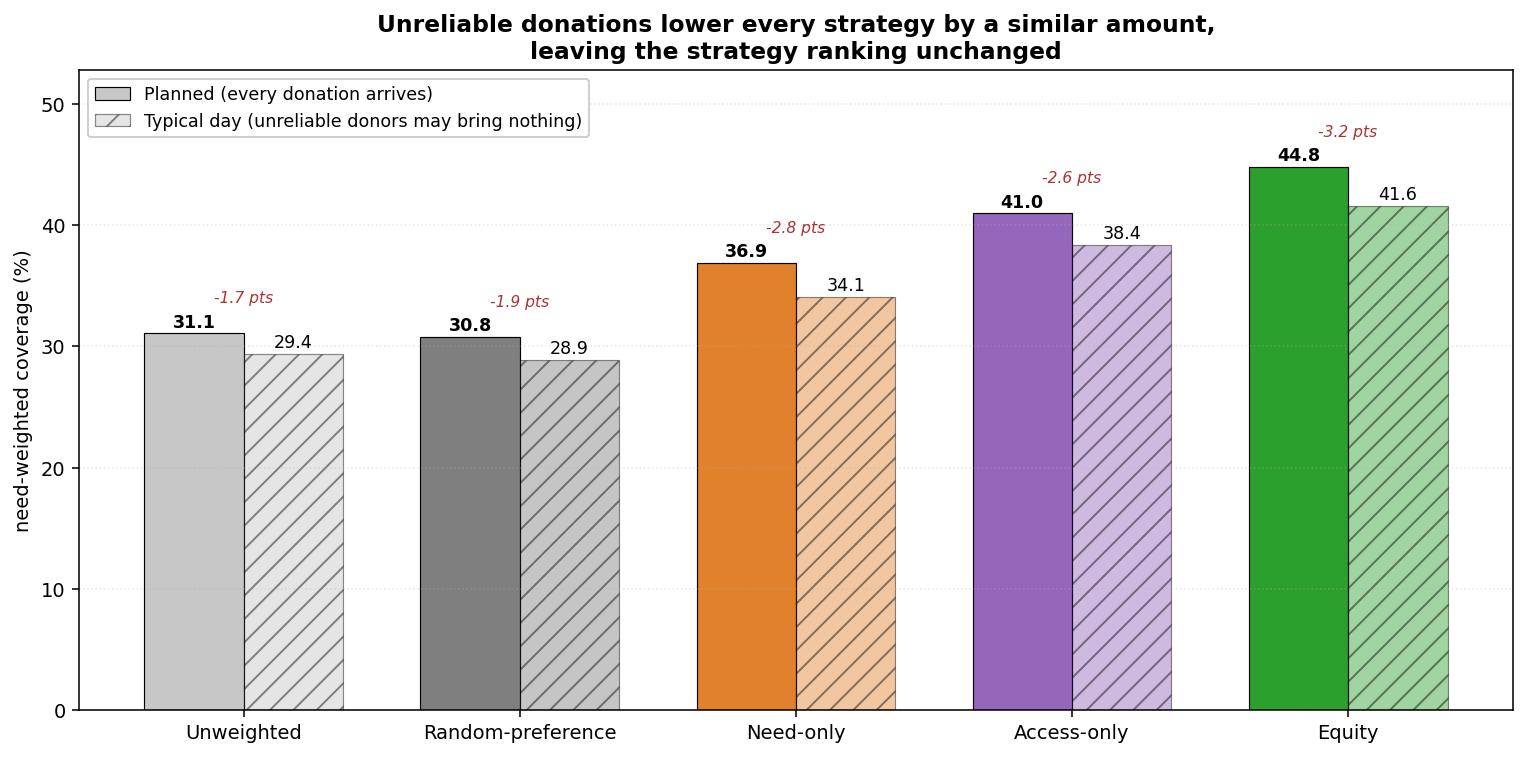
\includegraphics[width=0.92\linewidth,height=\textheight,keepaspectratio,alt={Donation uncertainty. For each strategy the solid bar is planned need-weighted coverage and the hatched bar is the mean realized coverage once unreliable donors are accounted for. The reduction is small and similar across strategies.}]{fig_blind_donations.png}
\caption{Donation uncertainty. For each strategy the solid bar is
planned need-weighted coverage and the hatched bar is the mean realized
coverage once unreliable donors are accounted for. The reduction is
small and similar across strategies.}
\end{figure}

\textbf{Data uncertainty.} We generated six scenarios that jointly
perturb demand (by 30 percent), travel times (by 15 percent), and
opening windows (by 20 minutes), and re-solved every strategy in each.
Point estimates shifted, but the central orderings were unchanged in the
six perturbation scenarios examined (Table 6, Figure 6). In all six, the
need-access strategy led on need-weighted coverage, and the need-only
strategy led on the highest-need tier. We treat this as evidence of
directional stability rather than a guarantee, and a larger uncertainty
study and multiple solver seeds are natural next steps.

\textbf{Table 6. Robustness across six perturbed scenarios (mean plus or
minus standard deviation).}

{\def\LTcaptype{none} % do not increment counter
\begin{longtable}[]{@{}
  >{\raggedright\arraybackslash}p{(\linewidth - 10\tabcolsep) * \real{0.1304}}
  >{\raggedleft\arraybackslash}p{(\linewidth - 10\tabcolsep) * \real{0.1739}}
  >{\raggedleft\arraybackslash}p{(\linewidth - 10\tabcolsep) * \real{0.1739}}
  >{\raggedleft\arraybackslash}p{(\linewidth - 10\tabcolsep) * \real{0.1739}}
  >{\raggedleft\arraybackslash}p{(\linewidth - 10\tabcolsep) * \real{0.1739}}
  >{\raggedleft\arraybackslash}p{(\linewidth - 10\tabcolsep) * \real{0.1739}}@{}}
\toprule\noalign{}
\begin{minipage}[b]{\linewidth}\raggedright
Metric
\end{minipage} & \begin{minipage}[b]{\linewidth}\raggedleft
Unweighted
\end{minipage} & \begin{minipage}[b]{\linewidth}\raggedleft
Random-pref.
\end{minipage} & \begin{minipage}[b]{\linewidth}\raggedleft
Need-only
\end{minipage} & \begin{minipage}[b]{\linewidth}\raggedleft
Access-only
\end{minipage} & \begin{minipage}[b]{\linewidth}\raggedleft
Need-access
\end{minipage} \\
\midrule\noalign{}
\endhead
\bottomrule\noalign{}
\endlastfoot
Recipients served & 229 ± 8 & 222 ± 8 & 198 ± 5 & 191 ± 6 & 184 ± 10 \\
Need-weighted coverage \% & 30.5 ± 0.8 & 30.0 ± 0.3 & 36.5 ± 0.8 & 40.4
± 1.4 & \textbf{44.2 ± 1.4} \\
High-need-tier coverage \% & 24.9 ± 1.1 & 26.0 ± 1.8 & \textbf{60.5 ±
1.9} & 23.9 ± 3.2 & 43.1 ± 2.7 \\
\end{longtable}
}

\begin{figure}
\centering
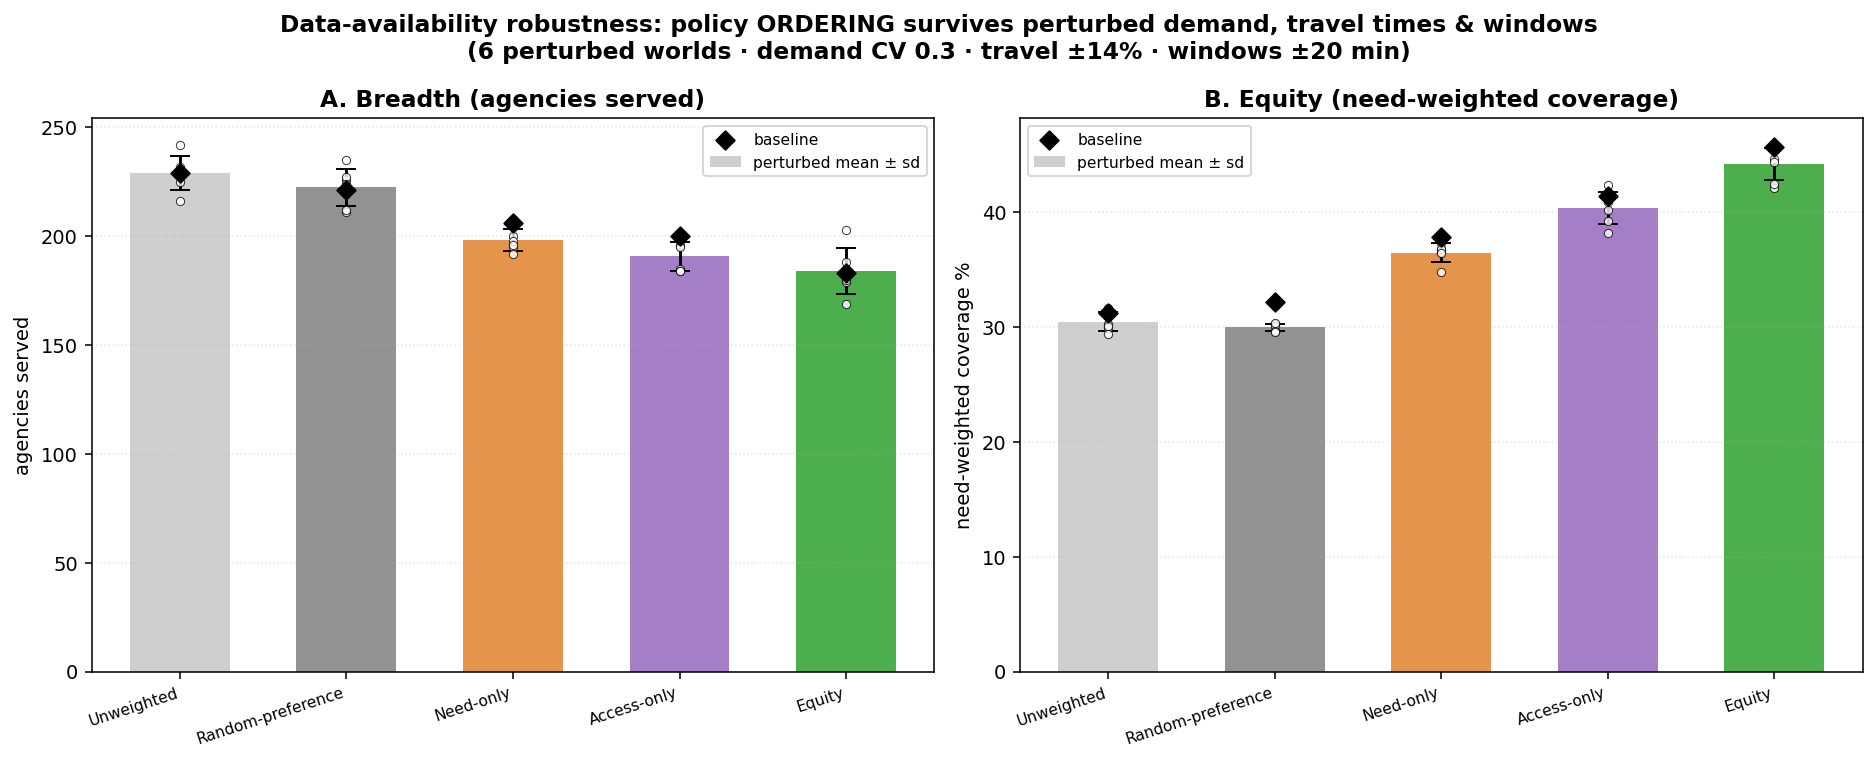
\includegraphics[width=0.92\linewidth,height=\textheight,keepaspectratio,alt={Robustness to data error. Bars show the mean over six perturbed scenarios with standard-deviation error bars; the unperturbed baseline is marked. The central orderings are preserved in every scenario examined.}]{robustness.png}
\caption{Robustness to data error. Bars show the mean over six perturbed
scenarios with standard-deviation error bars; the unperturbed baseline
is marked. The central orderings are preserved in every scenario
examined.}
\end{figure}

\section{6. Discussion}\label{discussion}

\textbf{Routing objectives encode distributive choices.} The central
result is structural rather than organizational. Under scarce capacity,
every routing objective induces a spatial distribution of service.
Neither benchmark without an equity signal serves high-need NYC
neighborhoods well: the unweighted benchmark, which is travel-efficient,
and the random-preference benchmark, which is not, both leave the
highest-need tier at roughly a quarter of its demand. Making need and
access explicit in the objective moves service toward disadvantaged
neighborhoods and, equally important, makes the size of that shift
measurable. Figure 3 shows the same point operationally: the unserved
recipients are a direct consequence of the objective, not an incidental
feature of the routes.

\textbf{Equity and adaptation are two responses to the same scarcity.}
The distributive choice studied here and the execution-time adaptation
set out in the three-layer model are not separate problems but two faces
of operating under scarce capacity. The objective decides who is served;
uncertainty then perturbs that allocation as the day unfolds. Our
results establish the first face, that an explicit need-and-access
objective measurably shifts service, and show that it is durable under
the donation-supply form of the second. The recipient-capacity recourse
layer formulated in Section 4.5 is where the two meet most sharply: when
an agency cannot accept a delivery, the recourse rule re-enacts the
distributive choice in miniature, deciding where the displaced food
goes. Quantifying that interaction is the natural next step, and the
commit-then-evaluate machinery already used for donation uncertainty
provides the seed for it.

\textbf{The choice of equity measure is itself a decision.} The ablation
shows that need and access capture different things. The combined ratio
maximizes need-weighted coverage, while a need-only objective best
serves the single neediest tier. A planner who treats access as part of
the definition of disadvantage will prefer the combined measure; a
planner who defines priority by raw need will prefer need-only. The
framework quantifies the consequences of each definition rather than
imposing one.

\textbf{Setting the dial is normative, not empirical.} The
diminishing-returns pattern in the gamma sweep means that, in this
instance, a moderate weighting captures most of the achievable equity
gain before reach erodes substantially. This can inform a decision, but
the appropriate setting expresses an organization's values and may
differ across networks.

\textbf{On the benchmarks.} We model the absence of an equity signal in
two distinct ways and do not assert that either reproduces current
practice. The value of the benchmarks is comparative: they show what
selection looks like when it is driven by logistics alone or by
arbitrary priorities, and that both fall well short of an explicit
equity objective.

\textbf{Modeled coverage is not realized impact.} Our outcomes are
modeled service-allocation measures. We do not measure household
receipt, nutritional adequacy, service frequency, substitution among
providers, spoilage after delivery, or beneficiary welfare. A model of
this kind can support exploratory analysis and strategic deliberation,
but operational implementation would require local calibration of
demand, capacity, service frequency, and food compatibility, and
downstream evaluation of realized outcomes.

\section{7. Limitations}\label{limitations}

Several limitations follow from the model's purpose as a strategic
decision-support tool.

Area-level need may not represent agency-level demand, and recipient
agencies differ in whom they serve. Provider count and opening hours
approximate provider capacity rather than measuring throughput, so the
access score is availability-based. Demand is estimated from operating
hours and published anchors rather than observed. The model treats a
single representative day and does not capture service rotation across
days, which would soften the apparent cost of any one day's unserved
locations. When a recipient is served the model delivers full demand
rather than a partial quantity, which can concentrate service; a
delivered-quantity objective with a concave utility or an explicit
per-tier service floor would mitigate the low coverage of low-priority
tiers and is a clear direction for future work. The adaptive layer as
evaluated covers donation-supply uncertainty only; recipient
receiving-capacity, its uncertainty, recourse, and split deliveries are
formulated within the three-layer model but are not enforced or
evaluated in the reported runs, and when added the recourse would be
simulated under an a-priori plan rather than fully optimized. The solver
is heuristic and reported under a fixed time budget, so values are not
guaranteed optimal, and we have not yet run multiple seeds. Priority
weights, the offset, and the clipping bounds encode normative and
modeling choices. Public data may be incomplete or outdated, and route
feasibility in the model is not the same as operational adoption.

\section{8. Conclusion}\label{conclusion}

When a New York City food-redistribution network cannot serve every
recipient, its routing model does not merely move food; it allocates a
scarce resource across an unequal landscape. We have shown, on an NYC
case network built from public locations and clearly labeled synthetic
parameters, that objectives without an equity signal, whether
travel-minimizing or arbitrary, produce similar spatial distributions
that do not favor high-need, low-access communities, and that an
explicit need-and-access objective shifts service toward those
communities by a measurable amount at a quantifiable cost in reach and
travel. An ablation clarifies that need and access contribute different
information, and a parameter sweep shows diminishing returns to stronger
equity weighting. These effects are directionally stable under the
demand, travel, window, and donation uncertainties we examined, and an
illustrative route map makes the distributive consequence visible: the
recipients a plan leaves unserved are chosen by its objective.

The contribution is a transparent framework, not a prescription. Routing
models do not eliminate value judgments; they formalize them. By making
the distributive consequences of an objective explicit and measurable,
such a framework lets a decision-maker choose deliberately, and evaluate
that choice, even when operational data is incomplete. Framing the
system as adaptive allocation also marks where the work goes next: the
same framework that makes the distributive choice explicit can make the
execution-time adaptation, recipient-capacity recourse above all,
explicit and measurable too.

\section{References}\label{references}

{[}1{]} R. Reusken et al., ``Optimization in food-bank supply chains
under data scarcity and capacity constraints,'' \emph{working reference,
strategic food-supply-chain design}.

{[}2{]} R. Nair et al., ``Scheduling and routing for food rescue with
uncertain donations and perishability,'' \emph{working reference,
operational food-rescue logistics}.

{[}3{]} I. S. Orgut, J. Ivy, R. Uzsoy, and J. R. Wilson, ``Modeling for
the Equitable and Effective Distribution of Donated Food under Capacity
Constraints,'' \emph{IIE Transactions}, 48(3), 2016.

{[}4{]} O. Eisenhandler and M. Tzur, ``The Humanitarian Pickup and
Distribution Problem,'' \emph{Operations Research}, 67(1), 2019.

{[}5{]} W. Luo and Y. Qi, ``An Enhanced Two-Step Floating Catchment Area
(E2SFCA) Method for Measuring Spatial Accessibility to Primary Care
Physicians,'' \emph{Health and Place}, 15(4), 2009.

{[}6{]} M. M. Solomon, ``Algorithms for the Vehicle Routing and
Scheduling Problems with Time Window Constraints,'' \emph{Operations
Research}, 35(2), 1987.

{[}7{]} P. Toth and D. Vigo (eds.), \emph{Vehicle Routing: Problems,
Methods, and Applications}, 2nd ed., SIAM, 2014.

{[}8{]} L. Perron and V. Furnon, \emph{OR-Tools}, Google.
https://developers.google.com/optimization

{[}9{]} Feeding America, \emph{Map the Meal Gap} (area-level
food-insecurity estimates). https://map.feedingamerica.org/

\emph{References {[}1{]} and {[}2{]} are the two reference papers
provided for this project; full bibliographic details, and the
feature-comparison entries in Table 1, should be verified against the
primary sources before submission.}

\section{Appendix A. Full constraint
set}\label{appendix-a.-full-constraint-set}

Using the notation of Section 4.6, with \(N = O \cup P \cup V\) and a
recipient served indicator \(y_i\):

\begin{itemize}
\tightlist
\item
  \textbf{Linking and degree.} For each recipient \(i \in V\),
  \(\sum_{k}\sum_{j} x_{jik} = y_i\) and
  \(\sum_{k}\sum_{j} x_{ijk} = y_i\). Donor visits are free and
  optional.
\item
  \textbf{Flow conservation.} For each node and vehicle, inflow equals
  outflow.
\item
  \textbf{Depot routes.} Each vehicle \(k\) departs from and returns to
  its depot.
\item
  \textbf{Capacity.} A load dimension accumulates donor supply \(s_p\)
  at pickups and subtracts demand \(d_i\) at deliveries, bounded above
  by \(Q_k\); a parallel cold-load dimension is bounded by \(Q^{c}_k\),
  so cold demand rides only on refrigerated vehicles.
\item
  \textbf{Time windows.} \(a_i \le \tau_i \le b_i\), with
  \(\tau_j \ge \tau_i + \text{service}_i + c_{ij}\) whenever arc
  \((i,j)\) is used, and total route duration within the working day.
\item
  \textbf{Perishability.} A soft penalty
  \(\delta\,\text{cold}_i\,\tau_i\) discourages late delivery of cold
  demand.
\end{itemize}

\section{Appendix B. Key parameters and
reproduction}\label{appendix-b.-key-parameters-and-reproduction}

{\def\LTcaptype{none} % do not increment counter
\begin{longtable}[]{@{}
  >{\raggedright\arraybackslash}p{(\linewidth - 4\tabcolsep) * \real{0.3333}}
  >{\raggedright\arraybackslash}p{(\linewidth - 4\tabcolsep) * \real{0.3333}}
  >{\raggedright\arraybackslash}p{(\linewidth - 4\tabcolsep) * \real{0.3333}}@{}}
\toprule\noalign{}
\begin{minipage}[b]{\linewidth}\raggedright
Parameter
\end{minipage} & \begin{minipage}[b]{\linewidth}\raggedright
Value
\end{minipage} & \begin{minipage}[b]{\linewidth}\raggedright
Note
\end{minipage} \\
\midrule\noalign{}
\endhead
\bottomrule\noalign{}
\endlastfoot
Recipients & 528 & public NYC locations \\
Donors & 18 (reliable plus uncertain) & per-donor availability and
variability \\
Vehicles & 25, about 70\% refrigerated, 2,500 lb each & scenario
parameter, two depots \\
Working day / service time & about 840 min / 15 min & from opening
hours \\
Total demand / cold share & about 104,000 lb / 44\% & synthetic, from
hours and public anchors \\
Deliverable per day & about 34,000 lb & roughly one third of demand \\
Priority weight &
\(\operatorname{clip}(((N+0.15)/(A+0.15))^{\gamma}, 0.5, 4)\) & gamma =
1 default; 128 distinct weights \\
Equity dial & gamma; diminishing returns past 0.5 to 1 in this instance
& normative \\
\end{longtable}
}

The supplementary scripts reproduce the strategy comparison, the
equity-dial sweep, the uncertainty analysis, and the illustrative route
map under a fixed solver time budget.

\end{document}
